\documentclass[article]{jss}
\usepackage[utf8]{inputenc}

\providecommand{\tightlist}{%
  \setlength{\itemsep}{0pt}\setlength{\parskip}{0pt}}

\author{
John Muschelli\\Department of Biostatistics, Johns Hopkins Bloomberg School of Public
Health
}
\title{ROC and AUC in R with a Binary Predictor}

\Plainauthor{John Muschelli}
\Plaintitle{ROC and AUC in R with a Binary Predictor}
\Shorttitle{Binary Predictor ROC}

\Abstract{
The abstract of the article.
}

\Keywords{roc, auc, area under the curve, \proglang{R}}
\Plainkeywords{roc, auc, area under the curve, R}

%% publication information
%% \Volume{50}
%% \Issue{9}
%% \Month{June}
%% \Year{2012}
%% \Submitdate{}
%% \Acceptdate{2012-06-04}

\Address{
    John Muschelli\\
  Department of Biostatistics, Johns Hopkins Bloomberg School of Public
  Health\\
  615 N Wolfe St Baltimore, MD 21205\\
  E-mail: \email{jmuschel@jhsph.edu}\\
  URL: \url{http://johnmuschelli}.\\~\\
  }

\usepackage{amsmath}

\begin{document}

\hypertarget{introduction}{%
\section{Introduction}\label{introduction}}

In many applications, receiver operator characteristic (ROC) curves are
used to show how a predictor compares to the true outcome. One of the
large draws of th ROC curve is that it is threshold-agnostic; it shows
the performace of a predictor without a specific threshold and also
gives a criteria to choose an optimal threshold based on a certain cost
function.

Many predictors, especially medical tests, result in a binary decision;
a value is higher than a pre-determined threshold or not. Similarly,
some are simply categorical or discrete; for example, blood pressure may
be low, normal, or high. These are useful indicators of presence
disease, which is a primary outcome of interest.

\citet{fawcett2006introduction} describes (in Fig. 6) how ties are
handled in a predictor. Ties are distinctly relevant for discrete and
binary predictors or models that predict a discrete number of values,
where many observations can have the same value/risk score. When drawing
the ROC curve, one can assume that all the ties do not correctly
classify the outcome (Fawcett called the ``pessimistic'' approach) or
that all the ties do correclty classify the outcome (called the
``optimistic'' approach). But Fawcett notes: \textgreater{} Any mixed
ordering of the instances will give a different set of step segments
within the rectangle formed by these two extremes. However, the ROC
curve should represent the \emph{expected} performance of the
classifier, which, lacking any other information, is the average of the
pessimistic and optimistic segments.

Therefore,

With some assumptions, you can think of the binary predictor as
generating from a distribution of values from a continuous distribution
that has been thresholded. Therefore, the sensitivity of this
thresholded predictor actually represents one point on the ROC curve of
the true underlying continuous distribution. Therefore the ROC curve of
a binary predictor is not really appropriate. But alas, ROC and AUC
analysis is done on binary predictors and used to inform if one variable
is more predictive than the other.

A more appropriate comparison of a continuous predictor and the binary
predictor may be to compare the sensitivity and specificity (or overall
accuracy) of the continuous predictor given the optimal threshold versus
that of the binary predictor.

This expectation directly applies to the assignment of a half
probability of success when the data are tied. This half probability is
linked to how ties are treated in the Wilcoxon rank sum test. As much of
the theory of ROC curve testing, and therefore testing of differences in
AUC, is based on the theory of the Wilcoxon rank-sum test, this
treatment of ties is relevant to statistical inference.

\begin{CodeChunk}

\begin{CodeInput}
R> library(cranlogs)
R> library(ggplot2)
R> library(dplyr)
\end{CodeInput}
\end{CodeChunk}

In this tutorial, we will show the calculation of the AUC

\hypertarget{simple-example}{%
\section{Simple Example}\label{simple-example}}

Here we will create a simple scenario where there is a binary predictor
\(X\) and a binary outcome \(Y\).\\

\begin{CodeChunk}

\begin{CodeInput}
R> x = c(rep(0, 52), rep(1, 32),
R+       rep(0, 35), rep(1, 50))
R> y = c(rep(0, 84), rep(1, 85))
R> tab = table(x, y)
R> tab
\end{CodeInput}

\begin{CodeOutput}
   y
x    0  1
  0 52 35
  1 32 50
\end{CodeOutput}
\end{CodeChunk}

\hypertarget{mathematical-proof-of-auc-for-single-binary-predictor}{%
\subsection{Mathematical Proof of AUC for Single Binary
Predictor}\label{mathematical-proof-of-auc-for-single-binary-predictor}}

As there are only two outcomes for \(X\), we can expand the probability
using the law of total probability: \begin{align}
P(X_{1} > X_{0}) &= P(X_{1} > X_{0} | X_{1} = 1) P(X_{1} = 1) \nonumber \\
&+ P(X_{1} > X_{0} | X_{1} = 0) P(X_{1} = 0) \label{eq:expand1} \\
&= P(X_{1} > X_{0} | X_{1} = 1) P(X_{1} = 1) \label{eq:expand}
\end{align} where the second term of equation \eqref{eq:expand1} is
equal to zero because \(X_{0} \in \{0, 1\}\).

Here we see that the second term of equation \eqref{eq:expand} is the
sensitivity: \begin{align*}
P(X_{1} = 1) &= P(X = 1 | Y = 1)\\
&= \frac{TP}{TP + FN} \\
&= \text{sensitivity}
\end{align*}

Here we show the first term of equation \eqref{eq:expand} is the
specificity: \begin{align*}
P(X_{1} > X_{0} | X_{1} = 1) &= P(X_{1} > X_{0} | X_{1} = 1, X_{0} =1) P(X_{0} = 1) \\
&+ P(X_{1} > X_{0} | X_{1} = 1, X_{0} =0) P(X_{0} = 0) \\
&= P(X_{1} > X_{0} | X_{1} = 1, X_{0} =0) P(X_{0} = 0) \\
&= P(X_{0} = 0) \\
&= P(X = 0 | Y = 0)\\
&= \frac{TN}{TN + FP} \\
&= \text{specificity}
\end{align*}

Therefore, we combine these two to show that equation \eqref{eq:expand}
reduces to: \[
P(X_{1} > X_{0}) = \text{specificity} * \text{sensitivity}
\]

Therefore, the true AUC should be equal to:
\textbackslash{}begin\{CodeChunk\}

\textbackslash{}begin\{CodeInput\} R\textgreater{} sens = tab{[}2,2{]} /
sum(tab{[},2{]}) R\textgreater{} spec = tab{[}1,1{]} / sum(tab{[},1{]})
R\textgreater{} true\_auc = sens * spec R\textgreater{} print(true\_auc)
\textbackslash{}end\{CodeInput\}

\begin{CodeOutput}
[1] 0.3641457
\end{CodeOutput}

\textbackslash{}end\{CodeChunk\}

\hypertarget{reverse-labeling}{%
\subsubsection{Reverse Labeling}\label{reverse-labeling}}

\textbackslash{}begin\{CodeChunk\}

\textbackslash{}begin\{CodeInput\} R\textgreater{} flip\_auc = (1 -
sens) * (1 - spec) R\textgreater{} print(flip\_auc)
\textbackslash{}end\{CodeInput\}

\begin{CodeOutput}
[1] 0.1568627
\end{CodeOutput}

\textbackslash{}end\{CodeChunk\}

\textbackslash{}begin\{CodeChunk\}

\textbackslash{}begin\{CodeInput\} R\textgreater{} fpr = 1-spec
R\textgreater{} area\_of\_tri = 1/2 * sens * fpr R\textgreater{}
area\_of\_quad = sens * spec + 1/2 * spec * (1-sens) R\textgreater{} auc
= area\_of\_tri + area\_of\_quad \textbackslash{}end\{CodeInput\}
\textbackslash{}end\{CodeChunk\}

We can also show that if we use a simple sampling method, we can
estimate this true AUC. Here, the function \code{est_auc} samples
10\^{}\{6\} random samples from \(X_{1}\) and \(X_{0}\), then calculates
\(\hat{P}(X_{1} > X_{0})\):

\textbackslash{}begin\{CodeChunk\}

\textbackslash{}begin\{CodeInput\} R\textgreater{} est\_auc =
function(x, y) \{ R+ x1 = x{[}y == 1{]} R+ x0 = x{[}y == 0{]} R+ n =
1000000 R+ c1 = sample(x1, size = n, replace = TRUE) R+ c0 = sample(x0,
size = n, replace = TRUE) R+ true\_auc = mean(c1 \textgreater{} c0) R+
\# calc\_auc = true\_auc + 1/2 * mean(c1 == c0) R+ \# c(true\_auc,
calc\_auc) R+ return(true\_auc) R+ \} R\textgreater{} sample\_est\_auc =
est\_auc(x, y) R\textgreater{} sample\_est\_auc
\textbackslash{}end\{CodeInput\}

\begin{CodeOutput}
[1] 0.364663
\end{CodeOutput}

\textbackslash{}end\{CodeChunk\}

\hypertarget{current-implementations}{%
\section{Current Implementations}\label{current-implementations}}

\hypertarget{r}{%
\subsection{R}\label{r}}

\hypertarget{catools-package}{%
\subsubsection{caTools Package}\label{catools-package}}

The \pkg{caTools} package is one of the most popular packages in R, and
has analysis for doing area under the curve:

\begin{CodeChunk}

\begin{CodeInput}
R> library(caTools)
R> colAUC(x, y)
\end{CodeInput}

\begin{CodeOutput}
             [,1]
0 vs. 1 0.6036415
\end{CodeOutput}
\end{CodeChunk}

\hypertarget{rocr-package}{%
\subsubsection{ROCR Package}\label{rocr-package}}

The \pkg{ROCR} package is one of the most popular packages for doing ROC
analysis \citep{ROCR}. Using \code{prediction} and \code{performance}
functions, we see that the estimated AUC is much higher than the true
AUC:

\textbackslash{}begin\{CodeChunk\}

\begin{CodeInput}
R> library(ROCR)
\end{CodeInput}

\begin{CodeOutput}
Loading required package: gplots
\end{CodeOutput}

\begin{CodeOutput}

Attaching package: 'gplots'
\end{CodeOutput}

\begin{CodeOutput}
The following object is masked from 'package:stats':

    lowess
\end{CodeOutput}

\textbackslash{}begin\{CodeInput\} R\textgreater{} pred = prediction(x,
y) R\textgreater{} auc\_est = performance(pred, ``auc'') R\textgreater{}
\href{mailto:auc_est@y.values}{\nolinkurl{auc\_est@y.values}}{[}{[}1{]}{]}
\textbackslash{}end\{CodeInput\}

\begin{CodeOutput}
[1] 0.6036415
\end{CodeOutput}

\textbackslash{}end\{CodeChunk\}

Looking at the plot for the ROC curve in ROCR, we can see why this may
be:

\begin{CodeChunk}

\begin{CodeInput}
R> par(mfrow = c(1, 2))
R> perf = performance(pred, "tpr", "fpr")
R> plot(perf)
R> abline(a = 0, b = 1)
R> plot(perf, type = "s")
R> abline(a = 0, b = 1)
\end{CodeInput}
\end{CodeChunk}

\begin{CodeChunk}


\begin{center}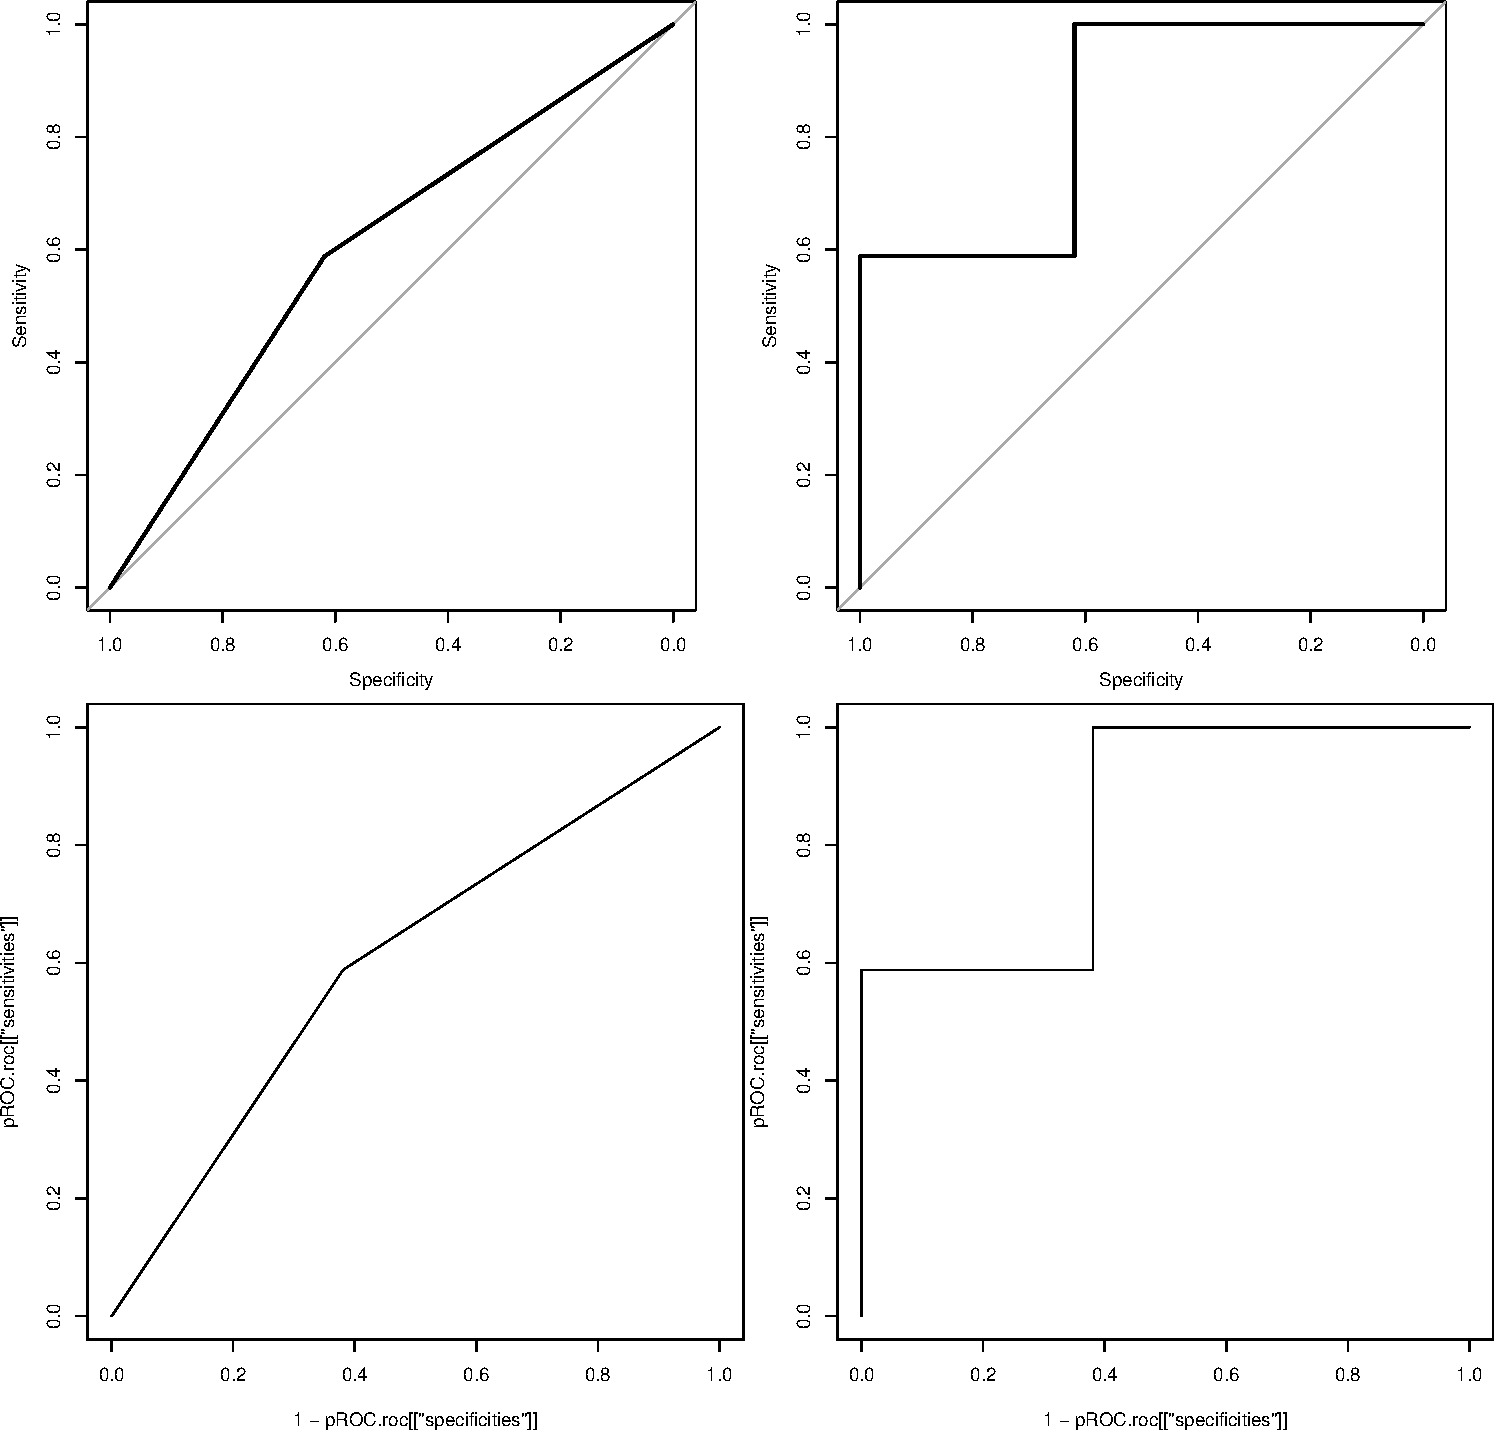
\includegraphics{index_files/figure-latex/unnamed-chunk-10-1} \end{center}

\end{CodeChunk}

Looking geometrically at the plot, we can see how
\textbackslash{}begin\{CodeChunk\}

\textbackslash{}begin\{CodeInput\} R\textgreater{} fpr = 1 - spec
R\textgreater{} area\_of\_left\_tri = 1/2 * sens * fpr R\textgreater{}
area\_of\_top\_tri = 1/2 * spec * (1 - sens) R\textgreater{} false\_auc
= area\_of\_left\_tri + true\_auc + area\_of\_top\_tri R\textgreater{}
false\_auc \textbackslash{}end\{CodeInput\}

\begin{CodeOutput}
[1] 0.6036415
\end{CodeOutput}

\textbackslash{}end\{CodeChunk\}

\hypertarget{proc-package}{%
\subsubsection{pROC Package}\label{proc-package}}

The \pkg{pROC} package is one of the most popular packages for doing ROC
analysis \citep{pROC}. Using \code{prediction} and \code{performance}
functions, we see that the estimated AUC is much higher than the true
AUC:

\textbackslash{}begin\{CodeChunk\}

\begin{CodeInput}
R> library(pROC)
\end{CodeInput}

\begin{CodeOutput}
Type 'citation("pROC")' for a citation.
\end{CodeOutput}

\begin{CodeOutput}

Attaching package: 'pROC'
\end{CodeOutput}

\begin{CodeOutput}
The following objects are masked from 'package:stats':

    cov, smooth, var
\end{CodeOutput}

\textbackslash{}begin\{CodeInput\} R\textgreater{} pROC\_roc =
pROC::roc(predictor = x, response = y) R\textgreater{}
pROC\_roc{[}{[}``auc''{]}{]} \textbackslash{}end\{CodeInput\}

\begin{CodeOutput}
Area under the curve: 0.6036
\end{CodeOutput}

\textbackslash{}end\{CodeChunk\}

\begin{CodeChunk}


\begin{center}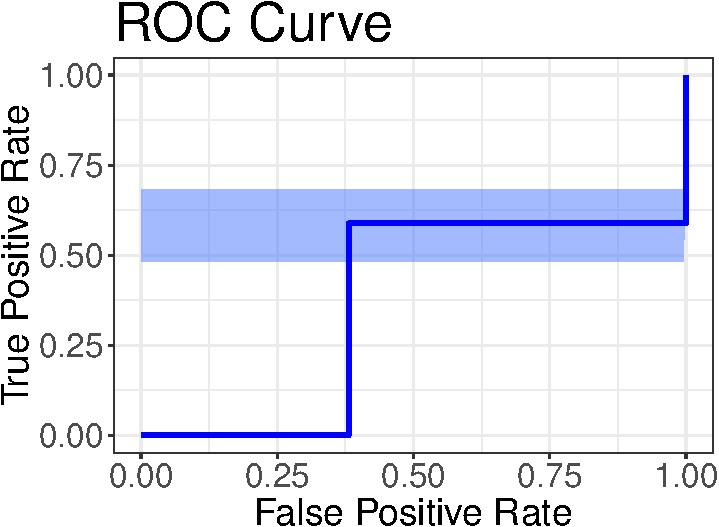
\includegraphics{index_files/figure-latex/unnamed-chunk-13-1} \end{center}

\end{CodeChunk}

\begin{CodeChunk}


\begin{center}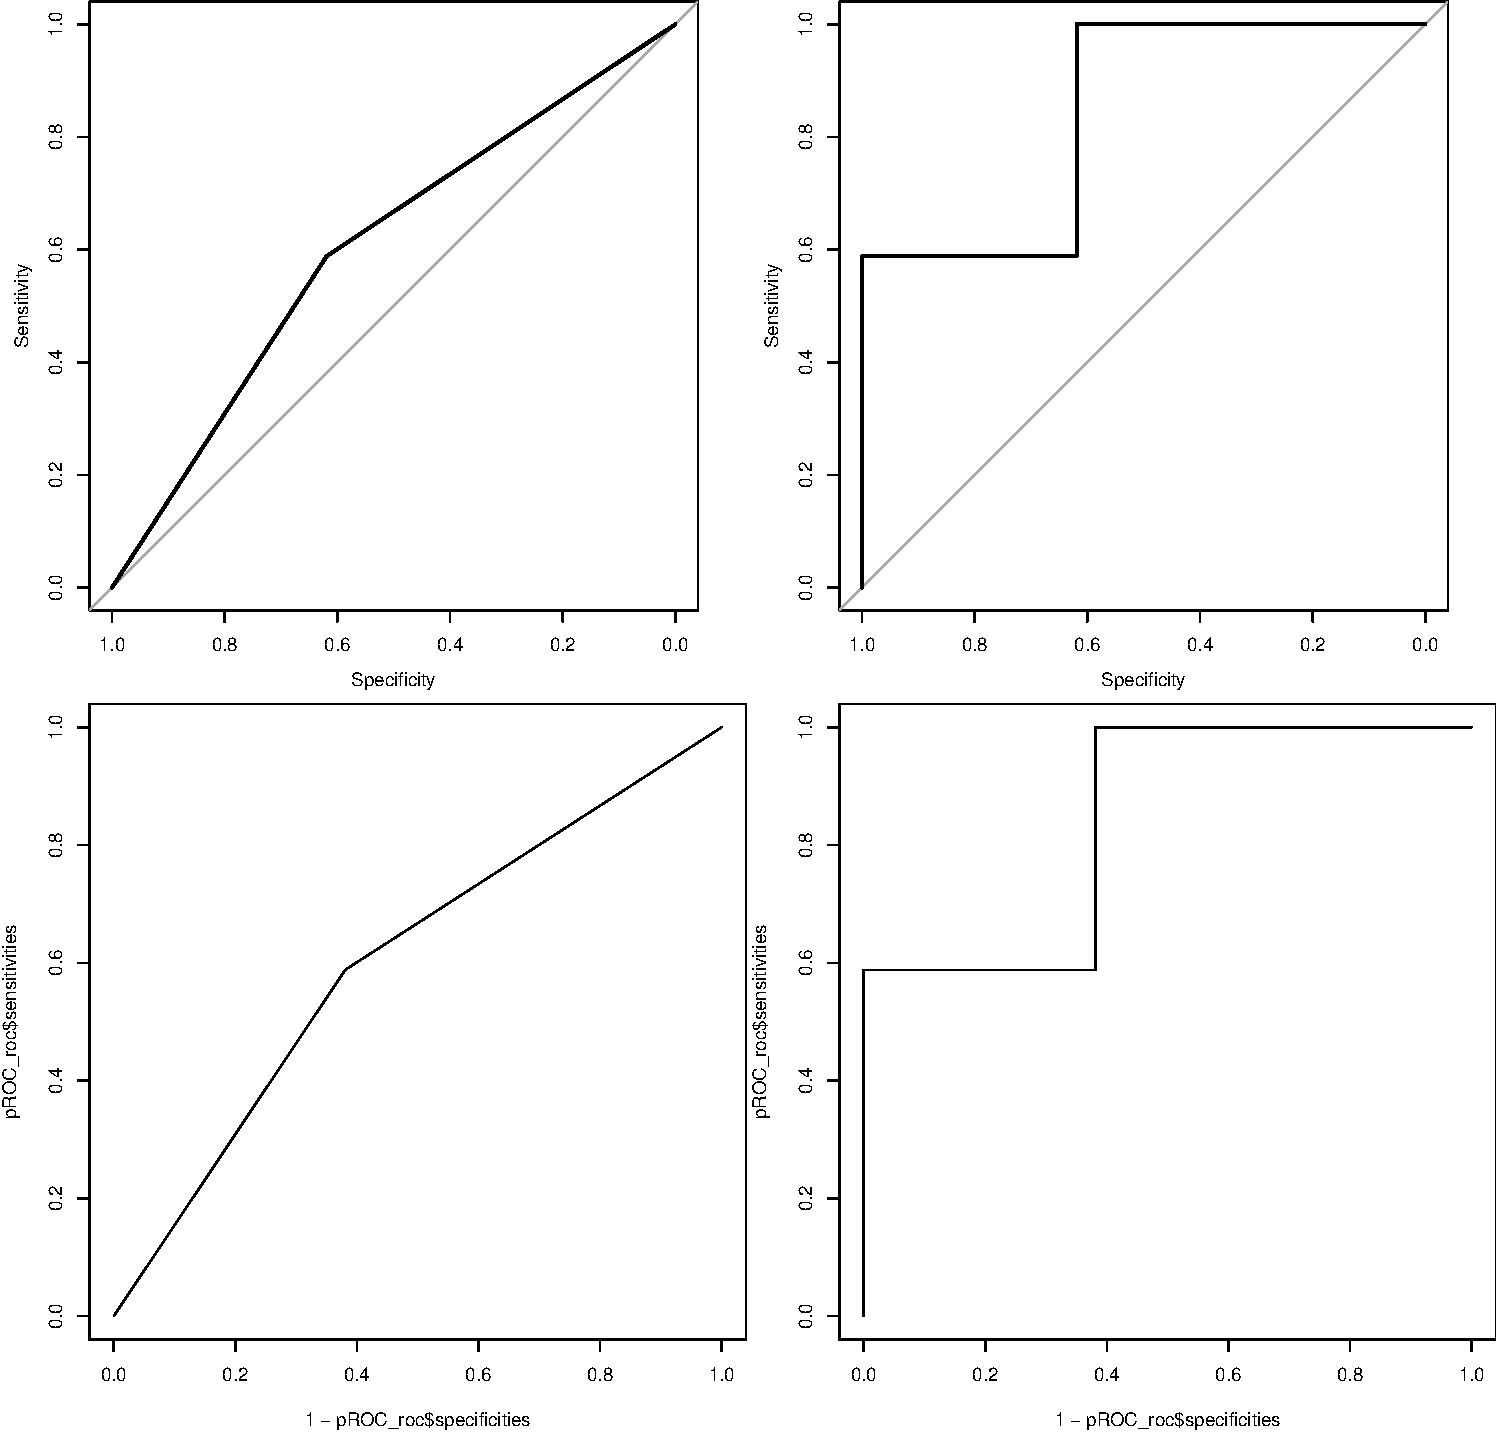
\includegraphics{index_files/figure-latex/unnamed-chunk-14-1} \end{center}

\end{CodeChunk}

\hypertarget{fbroc-package}{%
\subsubsection{fbroc Package}\label{fbroc-package}}

The \pkg{fbroc} package is one of the most popular packages for doing
ROC analysis \citep{fbroc}. Using \code{prediction} and
\code{performance} functions, we see that the estimated AUC is much
higher than the true AUC:

\textbackslash{}begin\{CodeChunk\}

\textbackslash{}begin\{CodeInput\} R\textgreater{} library(fbroc)
R\textgreater{} fb\_roc\_default = boot.roc(x, as.logical(y), n.boot =
1000, tie.strategy = 2) R\textgreater{} auc\_def =
perf(fb\_roc\_default, ``auc'') R\textgreater{}
auc\_def{[}{[}``Observed.Performance''{]}{]}
\textbackslash{}end\{CodeInput\}

\begin{CodeOutput}
[1] 0.6036415
\end{CodeOutput}

\textbackslash{}begin\{CodeInput\} R\textgreater{} fb\_roc\_alternative
= boot.roc(x, as.logical(y), n.boot = 1000, tie.strategy = 1)
R\textgreater{} auc\_alt = perf(fb\_roc\_alternative, ``auc'')
R\textgreater{} auc\_alt{[}{[}``Observed.Performance''{]}{]}
\textbackslash{}end\{CodeInput\}

\begin{CodeOutput}
[1] 0.6036415
\end{CodeOutput}

\textbackslash{}end\{CodeChunk\}

\begin{CodeChunk}


\begin{center}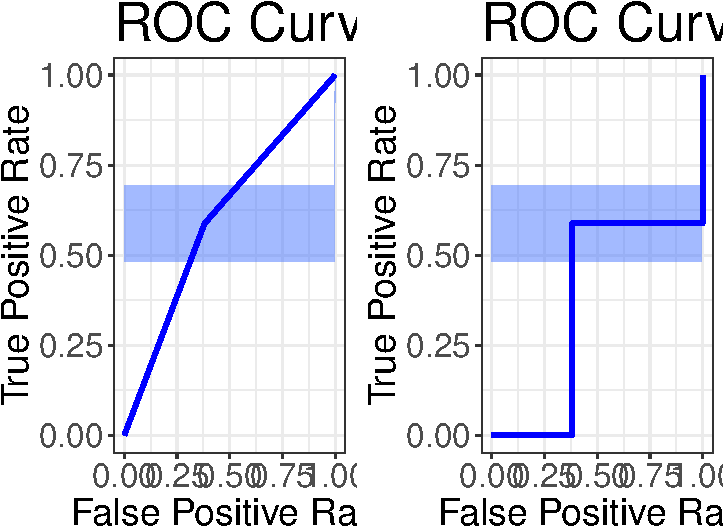
\includegraphics{index_files/figure-latex/unnamed-chunk-16-1} \end{center}



\begin{center}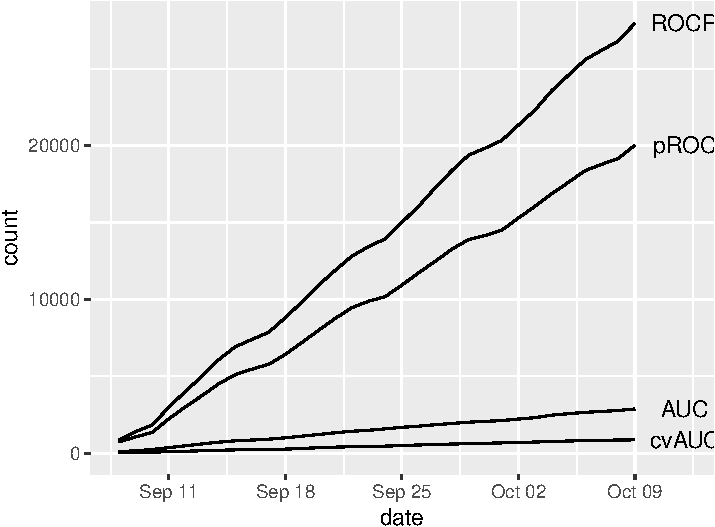
\includegraphics{index_files/figure-latex/unnamed-chunk-16-2} \end{center}

\end{CodeChunk}

\hypertarget{stata}{%
\subsection{Stata}\label{stata}}

\begin{CodeChunk}

\begin{CodeInput}
R> roctab x y
\end{CodeInput}


\begin{CodeOutput}
 . roctab x y

                      ROC                    -Asymptotic Normal--
           Obs       Area     Std. Err.      [95% Conf. Interval]
         --------------------------------------------------------
           169     0.6037       0.0379        0.52952     0.67793
\end{CodeOutput}
\end{CodeChunk}

\hypertarget{fawcett-example}{%
\subsection{Fawcett Example}\label{fawcett-example}}

\textbackslash{}begin\{CodeChunk\}

\begin{CodeInput}
R> faw = data.frame(y = c(rep(TRUE, 6), rep(FALSE, 4)),
R+                  x = c(0.99999, 0.99999, 0.99993, 
R+                        0.99986, 0.99964, 0.99955, 
R+                        0.68139, 0.50961, 0.48880, 0.44951))
R> faw$hyp = faw$x > 0.5
R> pred = prediction(predictions = faw$x, labels = faw$y)
R> par(mfrow = c(1, 2))
R> perf = performance(pred, "tpr", "fpr")
R> plot(perf)
R> abline(a = 0, b = 1)
R> plot(perf, type = "s")
R> abline(a = 0, b = 1)
\end{CodeInput}


\begin{center}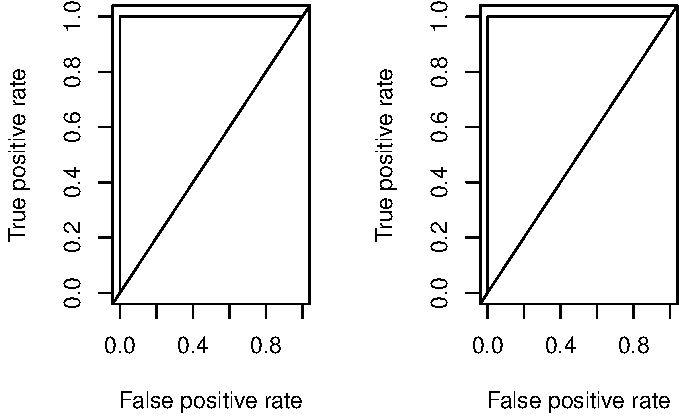
\includegraphics{index_files/figure-latex/fawcett-1} \end{center}

\textbackslash{}begin\{CodeInput\} R\textgreater{} auc\_est =
performance(pred, ``auc'') R\textgreater{}
\href{mailto:auc_est@y.values}{\nolinkurl{auc\_est@y.values}}{[}{[}1{]}{]}
\textbackslash{}end\{CodeInput\}

\begin{CodeOutput}
[1] 1
\end{CodeOutput}

\textbackslash{}begin\{CodeInput\} R\textgreater{} est\_auc(x =
faw\(x, y = faw\)y) \textbackslash{}end\{CodeInput\}

\begin{CodeOutput}
[1] 1
\end{CodeOutput}

\textbackslash{}end\{CodeChunk\}

\textbackslash{}begin\{CodeChunk\}

\textbackslash{}begin\{CodeInput\} R\textgreater{} library(dplyr)
R\textgreater{} fawcett = function(df) \{ R+ L\_sorted = df
\%\textgreater{}\% R+ arrange(desc(x), y) R+ n\_sample = nrow(L\_sorted)
R+ P = sum(L\_sorted{[}{[}``y''{]}{]}) R+ N = n\_sample - P R+ FP = TP =
0 R+ R = NULL R+ f\_prev = -Inf R+ i = 1 R+ for (i in seq(n\_sample)) \{
R+ f\_i = L\_sorted{[}{[}``x''{]}{]}{[}i{]} R+ if (f\_i != f\_prev) \{
R+ fpr = FP/N R+ tpr = TP / P R+ R = rbind(R, c(fpr = fpr, tpr = tpr))
R+ f\_prev = f\_i R+ \} R+ if
(L\_sorted\(y[i]) { R+ TP = TP + 1 R+ } R+ if (!L_sorted\)y{[}i{]}) \{
R+ FP = FP + 1 R+ \}\\
R+ \} R+ fpr = FP/N R+ tpr = TP / P R+ R = rbind(R, c(fpr = fpr, tpr =
tpr)) R+ return(R) R+ \} R\textgreater{} fawcett\_roc = fawcett(df)
R\textgreater{} seq\_range = function(x, \ldots{}) \{ R+ rx = range(x)
R+ seq(rx{[}1{]}, rx{[}2{]}, \ldots{}) R+ \} R\textgreater{} \#
seq\_range(faw\$x, ) \textbackslash{}end\{CodeInput\}
\textbackslash{}end\{CodeChunk\}

\bibliography{binroc.bib}


\end{document}

